%%%%%%%%%%%%%%%%%%%%%%%%%%%%%%%%%%%%%%%%%%%%%%%%%%%%%%%%%%%%%%%%%%%%
%% I, the copyright holder of this work, release this work into the
%% public domain. This applies worldwide. In some countries this may
%% not be legally possible; if so: I grant anyone the right to use
%% this work for any purpose, without any conditions, unless such
%% conditions are required by law.
%%%%%%%%%%%%%%%%%%%%%%%%%%%%%%%%%%%%%%%%%%%%%%%%%%%%%%%%%%%%%%%%%%%%

\documentclass{beamer}
\usetheme[faculty=fi]{fibeamer}
\usepackage[utf8]{inputenc}
\usepackage[
  main=english, %% By using `czech` or `slovak` as the main locale
                %% instead of `english`, you can typeset the
                %% presentation in either Czech or Slovak,
                %% respectively.
  				 %% The additional keys allow foreign texts to be
]{babel}   

%% These additional packages are used within the document:
\usepackage{ragged2e}  % `\justifying` text
\usepackage{booktabs}  % Tables
\usepackage{tabularx}
\usepackage{tikz}      % Diagrams
\usetikzlibrary{calc, shapes, backgrounds}
\usepackage{amsmath, amssymb}
\usepackage{url}       % `\url`s
\usepackage{listings}  % Code listings
\frenchspacing
\setbeamertemplate{frametitle}[default][center]
\begin{document}
  
 \begin{darkframes}
    \begin{frame}<beamer>
     \frametitle[alignment=center]{Tetris Attack}
      \begin{center}
		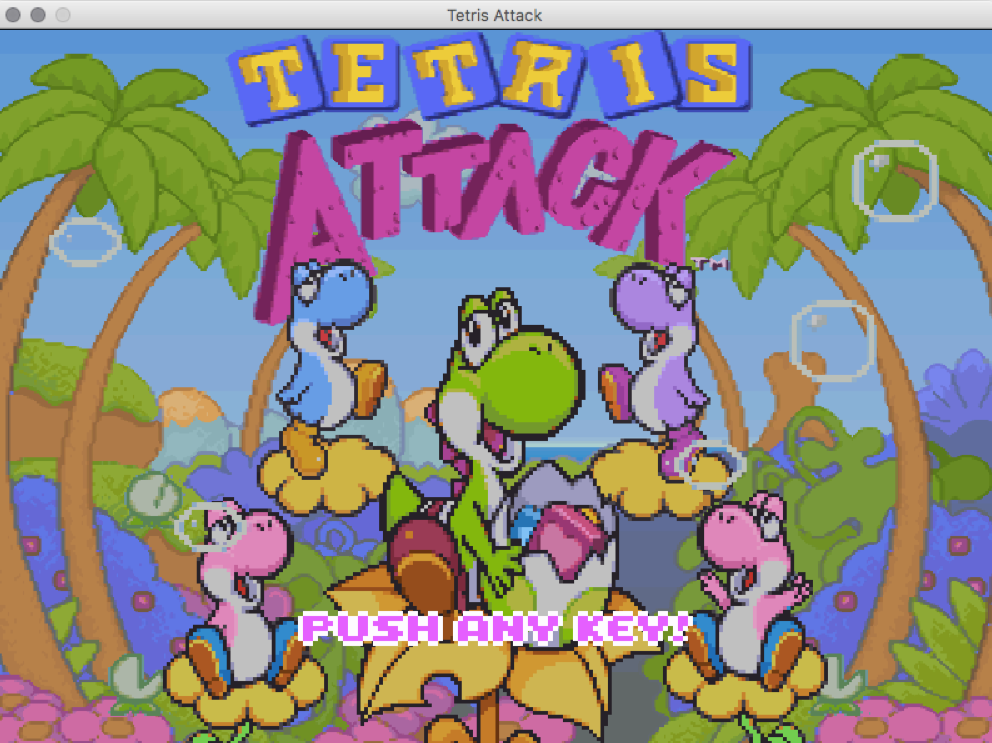
\includegraphics[scale=0.45]{./Image/img1.png}
		
		\end{center}
		\vspace*{0.1cm}
		  \begin{center}
		Valembois Vincent - Magniez Loick - Delabroye Kevin
		\end{center}
    \end{frame}

    \begin{frame}<beamer>
      \frametitle{Table des Matieres}
      \tableofcontents[]
    \end{frame}
    

 \section{Demonstation}
 \begin{frame}
 	 \frametitle{Démonstration}
 	 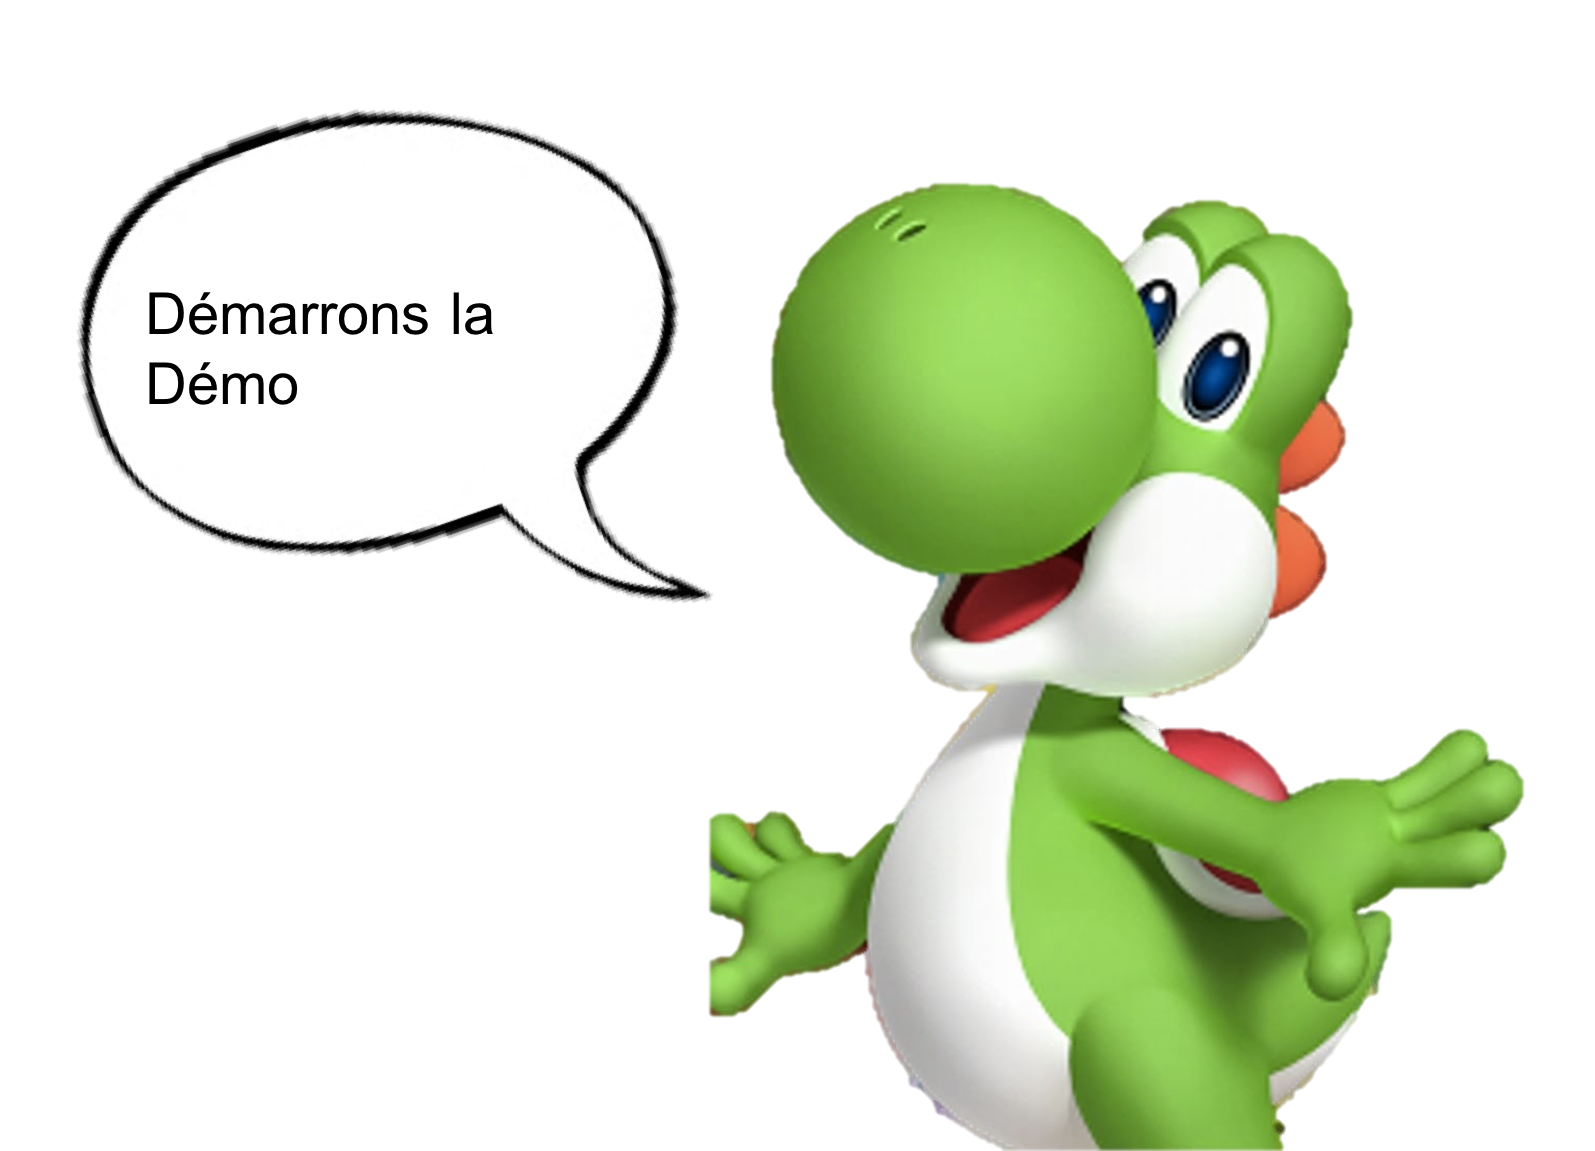
\includegraphics[scale=0.3]{./Image/demo.png}
    \end{frame}
    
 \section{Développement}
 \begin{frame}
 	 \frametitle{Développement}
 	 \begin{center}
 	 \framesubtitle{GIT}
 	 	Loïck : Animations, Menu, Événements du jeu \\%
 	 	Vincent : Modèle du jeu, Controler \\%
		Kévin : Contrôle du jeu, Menu \\%
 	 	
		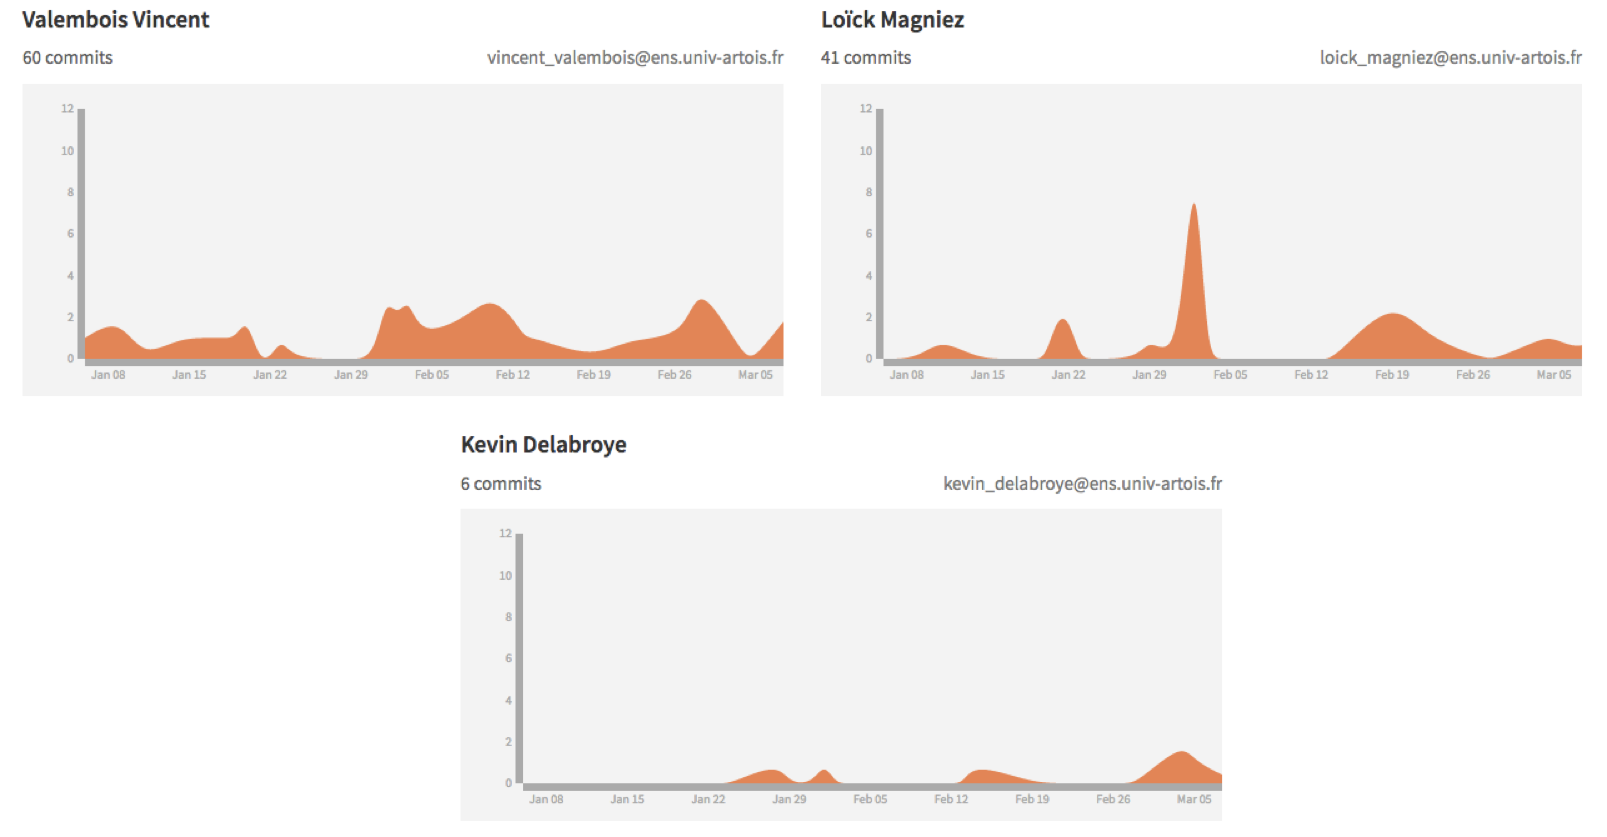
\includegraphics[scale=0.40]{./Image/git.png}
		\end{center}
    \end{frame}
    
     \begin{frame}
 	 \frametitle{Développement}
 	 \begin{center}
 	 \framesubtitle{UML}
 	 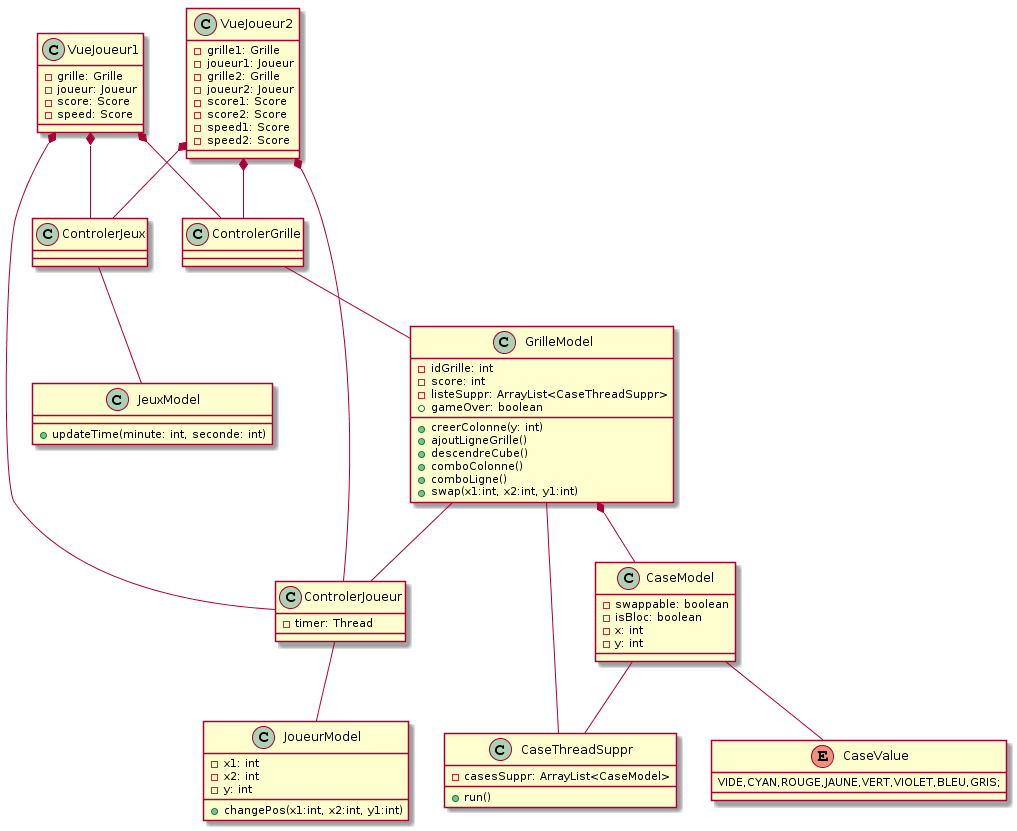
\includegraphics[scale=0.25]{./Image/diagramFinal.png}
		
		\end{center}
    \end{frame}
  
   \section{IHM}
 \begin{frame}
 	 \frametitle{IHM}
 	 \begin{center}
 	 \framesubtitle{Menu}
		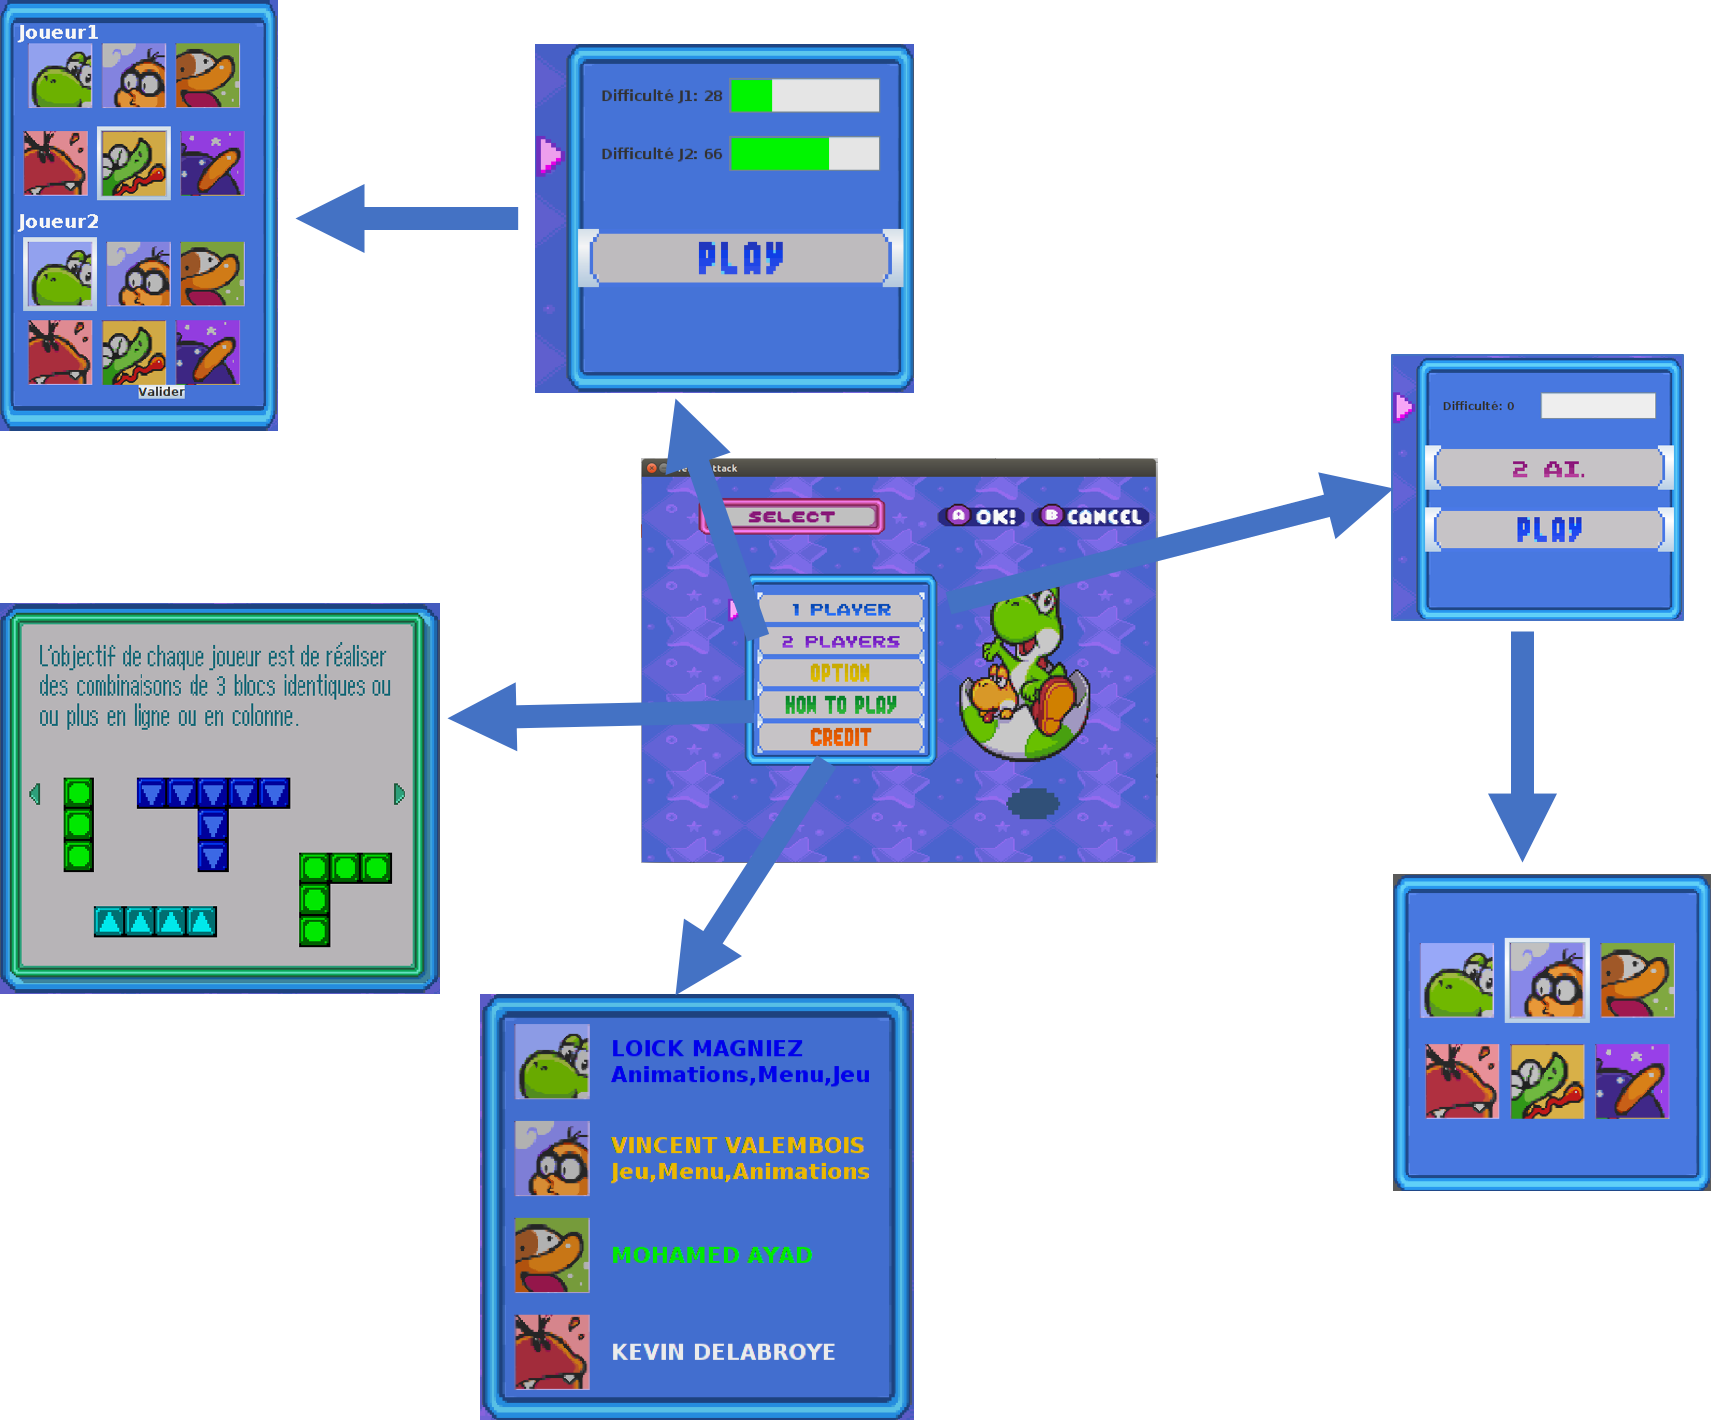
\includegraphics[scale=0.30]{./Image/arbo.png}
		\end{center}
    \end{frame}
    
         \begin{frame}
 	 \frametitle{IHM}
 	 \begin{center}
 	 \framesubtitle{Animation}
		
\includegraphics[scale=1.5]{./Image/jaune.png}\\%
		
\includegraphics[scale=1.0]{./Image/spriteSheet.png}
		\end{center}
    \end{frame}
    
    \begin{frame}
 	 \frametitle{IHM}
 	 \begin{center}
 	 \framesubtitle{Événements du jeu}
		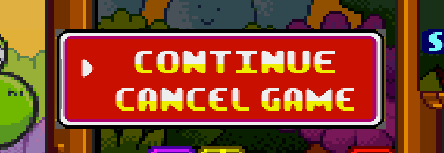
\includegraphics[scale=0.40]{./Image/pause.png}\\%
		
\includegraphics[scale=0.20]{./Image/gameOver.png}
		\end{center}
    \end{frame}
    
    \section{Fonctionnalite}
 \begin{frame}
 	 \frametitle{Fonctionnalite}
 	   \begin{enumerate}
    \item Jeu 1 joueur 
  \end{enumerate}
    \end{frame}
    
 \begin{frame}
 	 \frametitle{Fonctionnalite}
 	   \begin{enumerate}
    \item Jeu 1 joueur 
    \item Jeu Contre IA
  \end{enumerate}
    \end{frame}
    
 \begin{frame}
 	 \frametitle{Fonctionnalite}
 	   \begin{enumerate}
    \item Jeu 1 joueur 
    \item Jeu Contre IA
    \item Jeu 2 joueurs 
  \end{enumerate}
    \end{frame}
    
     \section{Evolution du Jeu}
 \begin{frame}
  \frametitle{Evolution du Jeu}
 	   \begin{enumerate}
    \item Ameliore IA
    \item Ajout des blocs Handicap
    
\includegraphics[scale=1.5]{./Image/brique.png}\\%
    \item Cubes exclamations
    
\includegraphics[scale=1.5]{./Image/grey.png}\\%
  \end{enumerate}
    \end{frame}


     \section{Les Difficultés}
 \begin{frame}
  \frametitle{Les Difficultés}
   	 \begin{center}
  
\includegraphics[scale=0.60]{./Image/difficulte.png}
  		\end{center}
    \end{frame}
    
         \section{Conclusion}
 \begin{frame}
   	 \begin{center}
  \Huge	 Conclusion
  		\end{center}
    \end{frame}
    
     \section{Les Questions}
 \begin{frame}
   	 \begin{center}
  	 \Huge	 Avez-vous des questions ?
  		\end{center}
    \end{frame}
    
  \end{darkframes}

\end{document}
